\section{Bài 3}

\subsection{Đề bài}
Ta thấy rằng $R_0$, thao tác phản xạ qua $\ket{0^n}$, có thể cài đặt như oracle pha $U_f$ với $f : \left\{ 0, 1 \right\}^n \to \left\{ 0, 1 \right\}$ được định nghĩa cho $x \in \left\{ 0, 1 \right\}^n$ là
\[
f(x) = \begin{cases}
0 \quad x = 0^n \\
1 \quad x \neq 0^n
\end{cases}
\]
Quan sát kỹ hơn, ta thấy $f$ chính là phép OR bit
\[
\operatorname{OR}(x_{n-1}\dots x_1x_0) = \sum_{i=0}^{n-1} x_i \mod 2.
\]
Như vậy bằng cách dùng các phiên bản lượng tử cho các cổng logic trong mạch logic cài đặt phép OR bit ta có thể cài đặt $R_0$. Cài đặt cụ thể $R_0$ theo cách này trong trường hợp $n=3$. Kiểm tra kết quả trên thư viện Qiskit.

\subsection{Lời giải}

Để cài đặt $R_0$ cho $n=3$, ta cần xây dựng mạch lượng tử thực hiện phép OR bit trên 3 qubit. Phép OR bit trên 3 qubit có thể được thực hiện bằng cách sử dụng các cổng Toffoli và CNOT. Dưới đây là mã Qiskit để cài đặt mạch này và kiểm tra kết quả.
\begin{lstlisting}[language=Python]
qc = QuantumCircuit(3)

qc.x([0, 1, 2])
qc.mcp(np.pi, [0, 1], 2)
qc.x([0, 1, 2])


print("\nVoi input |000>:")
vec_000 = Statevector.from_label("000").evolve(qc)
print(vec_000.draw("text"))

print("\nVoi input |001>:")
vec_001 = Statevector.from_label("001").evolve(qc)
print(vec_001.draw("text"))
\end{lstlisting}
Kết quả mạch lượng tử được vẽ như sau:
\begin{lstlisting}
Voi input |000>:
[-1.+0.j, 0.+0.j, 0.+0.j, 0.+0.j, 0.+0.j, 0.+0.j, 0.+0.j, 0.+0.j]

Voi input |001>:
[0.+0.00000000e+00j,1.-5.55111512e-17j,0.+0.00000000e+00j,
 0.+0.00000000e+00j,0.+0.00000000e+00j,0.+0.00000000e+00j,
 0.+0.00000000e+00j,0.+0.00000000e+00j]
\end{lstlisting}
Mạch lượng tử cài đặt $R_0$ cho $n=3$ được vẽ như sau:
\begin{figure}[H]
    \centering
    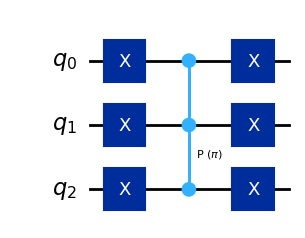
\includegraphics[width=0.3\textwidth]{img/section3_qc.png}
    \caption{Mạch lượng tử cài đặt $R_0$ cho $n=3$}
\end{figure}

Kết quả với đầu vào $\ket{000}$ là pha bị phản xạ (âm), trong khi với đầu vào $\ket{001}$ pha không bị thay đổi, đúng với định nghĩa của $R_0$. Tương tự, ta có thể kiểm tra với các đầu vào khác để xác nhận mạch hoạt động đúng.